% ============================================================
%  SCHOLA DOMESTICA MATHEMATICS — Level 1, Week 1, Lesson 1
%  Topic: Numbers 1 and 2 — Counting & Recognition
%  8 problems | No speed drill | Picture-heavy
%  Compile with XeLaTeX
% ============================================================

\documentclass[12pt, letterpaper]{article}
\usepackage[top=1in, bottom=1in, left=1in, right=1in]{geometry}
\usepackage{fontspec}
\usepackage{graphicx}
\usepackage{xcolor}
\usepackage{mdframed}
\usepackage{tikz}
\usetikzlibrary{shapes.geometric}
\usepackage{array}
\usepackage{tabularx}
\usepackage{microtype}
\usepackage{fancyhdr}
\usepackage{parskip}

\setmainfont{EB Garamond}[Ligatures=TeX, Numbers=OldStyle]
\newfontfamily\titlefont{EB Garamond}

\definecolor{sd-blue}{RGB}{60, 100, 160}
\definecolor{sd-gold}{RGB}{180, 140, 50}
\definecolor{sd-light}{RGB}{245, 242, 235}
\definecolor{sd-green}{RGB}{70, 130, 80}

\pagestyle{fancy}
\fancyhf{}
\renewcommand{\headrulewidth}{0.4pt}
\fancyhead[L]{\small\color{sd-blue}\textit{Schola Domestica Mathematics}}
\fancyhead[R]{\small\color{sd-blue}\textit{Level~1 \(\cdot\) Week~1 \(\cdot\) Lesson~1}}
\fancyfoot[C]{\small\color{sd-blue}1}

\newmdenv[backgroundcolor=sd-light,linecolor=sd-blue,linewidth=1pt,
  innerleftmargin=10pt,innerrightmargin=10pt,innertopmargin=8pt,
  innerbottommargin=8pt,roundcorner=4pt]{instructbox}

\newmdenv[backgroundcolor=white,linecolor=sd-green,linewidth=1.5pt,
  innerleftmargin=10pt,innerrightmargin=10pt,innertopmargin=8pt,
  innerbottommargin=8pt,roundcorner=4pt]{checkbox}

\newcommand{\ansblank}{\underline{\hspace{1.6cm}}}
\newcounter{probnum}
\newcommand{\prob}{\stepcounter{probnum}\noindent\textbf{\arabic{probnum}.}\quad}

% Draw a simple star using TikZ (fallback if star image missing)
\newcommand{\onestar}{%
  
\begin{tikzpicture}[baseline=-0.1cm]
    \node[star,star points=5,star point ratio=2.5,fill=sd-gold,
          draw=sd-gold!80!black,minimum size=1cm] {};
  \end{tikzpicture}}

% Draw a simple apple circle (fallback)
\newcommand{\oneapple}{%
  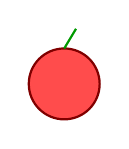
\begin{tikzpicture}[baseline=-0.1cm]
    \draw[fill=red!70, draw=red!50!black, thick] (0,0) circle (0.45cm);
    \draw[thick, green!60!black] (0,0.45) -- (0.15,0.7);
  \end{tikzpicture}}

\begin{document}

% ── Header ──────────────────────────────────────────────────
\begin{center}
  {\color{sd-blue}\Large\bfseries Schola Domestica Mathematics — Level~1}\\[4pt]
  {\color{sd-blue}\rule{\linewidth}{1.5pt}}\\[6pt]
  {\LARGE\bfseries Lesson 1 \quad|\quad Numbers 1 and 2}\\[4pt]
  {\color{sd-gold}\rule{\linewidth}{0.8pt}}
\end{center}

\vspace{4pt}

% ── Instruction ─────────────────────────────────────────────
\begin{instructbox}
\noindent\textbf{\color{sd-blue}Instruction} \textit{(read aloud to your student):}\\[4pt]
Today we will learn the numbers \textbf{1} and \textbf{2}.
When you count one thing, you say \textbf{one}.
When you count two things, you say \textbf{two}.
Let us count together!
\end{instructbox}

\vspace{10pt}

% ── Trace Block ─────────────────────────────────────────────
\noindent\textbf{\color{sd-blue}Trace and write:}

\vspace{6pt}
\begin{center}
\begin{tabular}{|c|c|c|c|c|c|}
\hline
\rule{0pt}{28pt}
{\Huge\color{sd-blue!40} 1} &
{\Huge\phantom{1}} &
{\Huge\phantom{1}} &
{\Huge\color{sd-blue!40} 2} &
{\Huge\phantom{2}} &
{\Huge\phantom{2}} \\
\hline
\end{tabular}
\end{center}

\vspace{8pt}
{\color{sd-gold}\rule{\linewidth}{0.5pt}}
\vspace{8pt}

% ── Practice Problems ────────────────────────────────────────
\noindent\textbf{\color{sd-blue}Practice}

\vspace{6pt}

\prob Count the stars. How many? \quad
% Use image if available; TikZ fallback shown
\IfFileExists{stars_1.jpg}{%
  
\includegraphics[height=1.4cm]{stars_1.jpg}}{%
  \onestar}%
\quad \ansblank

\vspace{10pt}

\prob Count the apples. How many? \quad
\IfFileExists{apples_2.jpg}{%
  
\includegraphics[height=1.4cm]{apples_2.jpg}}{%
  \oneapple\quad\oneapple}%
\quad \ansblank

\vspace{10pt}

\prob Circle the group that has \textbf{1}.

\vspace{6pt}
\begin{center}
\begin{tabular}{ccc}
\IfFileExists{ducks_1.jpg}{%
  
\includegraphics[height=1.6cm]{ducks_1.jpg}}{%
  
\begin{tikzpicture}
    \draw[fill=yellow!70,thick] (0,0) ellipse (0.4 and 0.3);
  \end{tikzpicture}}
&\quad\quad&
\IfFileExists{ducks_2.jpg}{%
  
\includegraphics[height=1.6cm]{ducks_2.jpg}}{%
  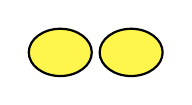
\begin{tikzpicture}
    \foreach \x in {0,0.9} \draw[fill=yellow!70,thick] (\x,0) ellipse (0.4 and 0.3);
  \end{tikzpicture}}
\\[4pt]
\textbf{A} && \textbf{B}
\end{tabular}
\end{center}

\vspace{10pt}

\prob Circle the group that has \textbf{2}.

\vspace{6pt}
\begin{center}
\begin{tabular}{ccc}
\IfFileExists{blocks_2.jpg}{%
  \includegraphics[height=1.6cm]{blocks_2.jpg}}{%
  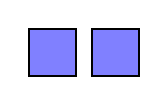
\begin{tikzpicture}
    \foreach \x in {0,0.8} \draw[fill=blue!50,thick] (\x,0) rectangle (\x+0.6,0.6);
  \end{tikzpicture}}
&\quad\quad&
\IfFileExists{blocks_1.jpg}{%
  \includegraphics[height=1.6cm]{blocks_1.jpg}}{%
  
\begin{tikzpicture}
    \draw[fill=blue!50,thick] (0,0) rectangle (0.6,0.6);
  \end{tikzpicture}}
\\[4pt]
\textbf{A} && \textbf{B}
\end{tabular}
\end{center}

\vspace{10pt}

\prob \textit{(Teacher reads aloud)} There is \textbf{1} rabbit in the garden.
Then \textbf{1} more rabbit hops in.
How many rabbits are there now? \quad \ansblank

\vspace{10pt}

\prob Draw \textbf{1} circle in the box.

\vspace{4pt}
\noindent\fbox{\rule{0pt}{2.5cm}\hspace{8cm}}

\vspace{10pt}

\prob Draw \textbf{2} stars in the box.

\vspace{4pt}
\noindent\fbox{\rule{0pt}{2.5cm}\hspace{8cm}}

\vspace{10pt}

\prob How many fingers am I holding up?\quad
\IfFileExists{fingers.jpg}{%
  \includegraphics[height=2cm]{fingers.jpg}}{%
  \textit{[Teacher holds up 2 fingers]}}
\quad \ansblank

\vspace{8pt}
{\color{sd-gold}\rule{\linewidth}{0.6pt}}
\vspace{6pt}

% ── Knowledge Check ─────────────────────────────────────────
\begin{checkbox}
\noindent\textbf{\color{sd-green}Knowledge Check}\\[4pt]
\textit{Mastery: student answers both correctly without hesitation.}\\[6pt]
\setcounter{probnum}{0}
\prob Point to the number \textbf{1}. \quad
  {\Large\quad\textbf{2}\quad\quad\textbf{1}\quad\quad\textbf{3}}\\[8pt]
\prob How many? \quad
  \IfFileExists{stars_2.jpg}{%
    
\includegraphics[height=1.2cm]{stars_2.jpg}}{%
    \onestar\onestar}%
  \quad \ansblank
\end{checkbox}

\vfill

% ── Enrichment ───────────────────────────────────────────────
\noindent{\color{sd-blue}$\bigstar$ \textbf{Enrichment:}}
In Latin, one is \textit{ūnus} and two is \textit{duo}.
Say them aloud: \textit{ūnus}, \textit{duo}!

\vspace{6pt}
\hrule
\vspace{4pt}
{\footnotesize\color{gray}\textit{Teacher note: Use real objects (acorns, buttons, coins)
to reinforce 1 and 2 before written work.
If student is not yet writing, allow pointing or oral answers for all problems.}}

\end{document}
